\documentclass{beamer}

\usepackage[utf8]{inputenc}
\usepackage{default}


\usepackage{multirow} %for aligning stuff in tables

\usepackage{bbding} %for the smiley face

\usepackage{calc} %calculate spacing \widthof

%tikz stuff
\usepackage{tikzsymbols}
\usepackage{tikz}
\usetikzlibrary{fit,arrows,positioning}

  % Keys to support piece-wise uncovering of elements in TikZ pictures:
  % \node[visible on=<2->](foo){Foo}
  % \node[visible on=<{2,4}>](bar){Bar}   % put braces around comma expressions
  %
  % Internally works by setting opacity=0 when invisible, which has the 
  % adavantage (compared to \node<2->(foo){Foo} that the node is always there, hence
  % always consumes space plus that coordinate (foo) is always available.
  %
  % The actual command that implements the invisibility can be overriden
  % by altering the style invisible. For instance \tikzsset{invisible/.style={opacity=0.2}}
  % would dim the "invisible" parts. Alternatively, the color might be set to white, if the
  % output driver does not support transparencies (e.g., PS) 
  %
  \tikzset{
    invisible/.style={opacity=0},
    visible on/.style={alt={#1{}{invisible}}},
    alt/.code args={<#1>#2#3}{%
      \alt<#1>{\pgfkeysalso{#2}}{\pgfkeysalso{#3}} % \pgfkeysalso doesn't change the path
    },
  }
  \tikzset{
    dimmed/.style={opacity=0.2},
    dimmed on/.style={alt={#1{dimmed}{}}},
    alt/.code args={<#1>#2#3}{%
      \alt<#1>{\pgfkeysalso{#2}}{\pgfkeysalso{#3}} % \pgfkeysalso doesn't change the path
    },
  }
\tikzset{
    %Define standard arrow tip
    >=stealth',
    %Define style for boxes
    peer/.style={
           rectangle,
           rounded corners,
           draw=black, thin,
           text width=3.5em,
           minimum height=2em,
           text centered},
    node/.style={
           rectangle,
           rounded corners,
           draw=black, 
           text width=4.5em,
           minimum height=2em,
           text centered,
           fill={rgb:black,1;white,3}},
    chunk/.style={
           rectangle,
           rounded corners,
           draw=black, 
           text width=2.5em,
           minimum height=1em,
           text centered,
           fill=block title bg},
    % Define arrow style
    point/.style={
           ->,
           thick,
           shorten <=2pt,
           shorten >=2pt,}
every node/.style={align=center}           
}

\newcommand{\wholeslide}[2][]{
\begin{frame}{#1}
% \transboxout<1>[duration=0.5]
\setbeamercolor{bgcolor}{fg=black,bg=white}
\begin{tikzpicture}[overlay, remember picture]
\node[anchor=center] at (current page.center) {
  \begin{beamercolorbox}[center]{bgcolor}
     #2
  \end{beamercolorbox}};
\end{tikzpicture}

\end{frame}
}

\newcommand{\blankslide}[2][]{
\begin{frame}[plain]{#1}
% \transboxout<1>[duration=0.5]
\setbeamercolor{bgcolor}{fg=black,bg=white}
\begin{tikzpicture}[overlay, remember picture]
\node[anchor=center] at (current page.center) {
  \begin{beamercolorbox}[center]{bgcolor}
     #2
  \end{beamercolorbox}};
\end{tikzpicture}

\end{frame}
}

\newenvironment<>{varblock}[2][.9\textwidth]{%
  \setlength{\textwidth}{#1}
  \begin{actionenv}#3%
    \def\insertblocktitle{#2}%
    \par%
    \usebeamertemplate{block begin}}
  {\par%
    \usebeamertemplate{block end}%
  \end{actionenv}}

\newlength{\mywidth}
\newcommand{\blockslide}[3][]{
\settowidth{\mywidth}{#3}
\begin{frame}[c]{#1}
\begin{center}
\begin{minipage}{1.1\mywidth}
 \begin{varblock}[1.1\mywidth]{#2}
  #3
 \end{varblock}
\end{minipage}
\end{center}
\end{frame}
}

\mode<presentation>{
\usetheme{Warsaw}\usecolortheme{crane}
\setbeamertemplate{items}[square]
\setbeamertemplate{section in toc}[square]
\setbeamertemplate{subsection in toc}[square]
% \setbeamertemplate{subsection in toc}[subsections numbered]
\setbeamertemplate{subsubsection in toc}[square]
% \setbeamercolor{items}{fg=black,bg=yellow}
\usebeamercolor{block title}
\definecolor{block title bg}{named}{bg}
\setbeamercolor{item projected}{fg=black,bg=block title bg}
\setbeamercolor{itemize item}{fg=block title bg,bg=block title bg}
}







\title{The rise of the third web}
\author{Viktor Tron and Aron Fischer}

\AtBeginSection[]
{
\begin{frame}<beamer>
\frametitle{Outline}
\tableofcontents[currentsection,sectionstyle=show/shaded,subsectionstyle=show/show/hide,subsubsectionstyle=show/show/show/hide]
\end{frame}
}

\begin{document}

\begin{frame}
 \titlepage
\end{frame}

\blankslide{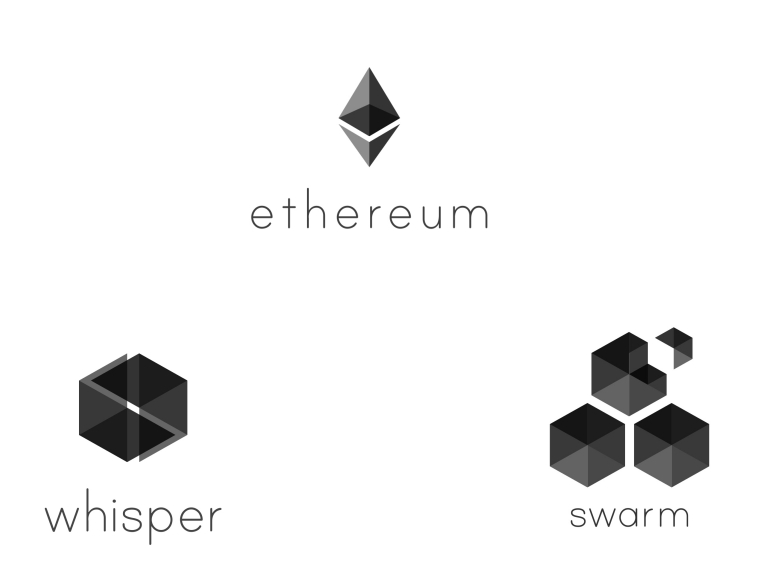
\includegraphics[width=0.8\textwidth]{ecosystem0.jpg}} 

\begin{frame}
 \tableofcontents[subsectionstyle=shaded/shaded,subsubsectionstyle=hide/hide]
\end{frame}

\begin{frame}
 Combining the power of the blockchain with a decentralised content storage and delivery network.
\end{frame}

\begin{section}{Content Delivery}

\subsection{Data Retrieval}
\blockslide{\textbf{Data out}}{How to retrieve data stored in the swarm.}


\begin{frame}{Data Retrieval}
\begin{columns}[T]
\begin{column}{0.4\textwidth}
\small
\alt<1-3>{}{\tiny}{
Everything on the swarm network has an \textbf<1-3>{id}, every chunk of data, every node (even you!). The \textbf<1-3>{id} also functions as an \textbf<1-3>{address}.\\[5mm]
}
\uncover<4->{\alt<4-5>{\small}{\tiny}
When your swarm-enabled dapp wishes to retrieve ``awesome-swarm-slides.pdf'',}
\uncover<5->{\alt<5>{}{\tiny}{it will attempt to retrieve it via its id ``\textbf{H}''.\\[5mm]
}}
\uncover<6->{\alt<6>{\small}{\tiny}
{
In swarm, the content with address ``\textbf{H}'' is stored with the node whose own address is \emph{closest} to \textbf{H}.\\[5mm]
}}
\uncover<7->{\alt<7>{\small}{\tiny}
{
Swarm's \textbf<7>{Retrieval Process} is responsible for deliviering the data to you.
}}
\end{column}

\begin{column}{0.6\textwidth} 
\begin{tikzpicture}
 \node[scale=0.7]{
    \begin{tikzpicture}
      \node[visible on=<2->] at (2,2) {\textbf{The Swarm Network:}};
      
      \node[node,visible on=<2->] at (0,0) {};
      \node[node,visible on=<2->] at (1,-0.9) {};
      \node[node,visible on=<2->] at (0.5,-3) {};
      \node[node,visible on=<2->] at (0,-6.3) {};
      \node[node,visible on=<2->] at (5.8,-1.2) {};
      \node[node,visible on=<2->] at (4,-5.9) {};
      \node[node,visible on=<2->] at (4.1,-3) {};
      \node[node,visible on=<2->] at (2.1,-2) {};

      \node[node,visible on=<2>] at (4,0) (younode) {swarm-node};
      \node[peer,visible on=<3->] at (4,0) (you) {You};
      
      \node[visible on=<5->] (chunk) at (1,-5) {$\bullet$};
      \node[visible on=<5->] (chunklabel) at (2,-4.5) {H} edge[point,->,visible on =<5->] (chunk);

      \node[visible on=<2-6>, node] at (-0.5,-4.2) (close) {};
      \node[visible on=<7->, peer] at (-0.5,-4.2) (closestnode) {Closest Node};
      \node[visible on=<7->] at (-0.5, -5.5) (hlabel) {Look for ``H'' here} 
	  edge[visible on=<7->,point,->] (closestnode);
    \end{tikzpicture}
    };
\end{tikzpicture}
\end{column}
\end{columns}

\end{frame}






\begin{frame}{Swarm Retrieval Process}
 
\begin{tikzpicture}
\node[peer,visible on=<1->] at (12,0) (retriever){Retriever};
\node[visible on=<13>,scale=2] at (12,-1.5) {\Smiley};

\node[visible on=<2->] (chunk) at (4,-5) {$\bullet$};
\node[visible on=<2->] (chunklabel) at (3,-4) {data address} edge[point,->,visible on =<2->] (chunk);

\node[peer,visible on=<4-12>, dimmed on=<13->] at (8.5,-0.5) (connectedpeer){peer}
    (retriever.-150) edge[point, ->,visible on=<5>,dimmed on=<6-12>,  bend left=15] 
	    node[below=2pt,visible on=<5>, dimmed on=<6-12>] {request}
		    (connectedpeer.-10);
		    
\node[node,visible on=<6-11>, dimmed on=<12->] at (6,-2) (firstnode){some node}
	(connectedpeer.-70) edge[point,->,visible on=<6>, dimmed on=<7-11>,bend left=30] 
	    node[right of=2pt,visible on=<6>, dimmed on=<7-11>] {request} 
		    (firstnode.east);

\node[node,visible on=<7-10>, dimmed on=<11->] at (7.5,-4.5) (secondnode){other node}
	(firstnode.-70) edge[point,->,dashed,visible on=<7>, dimmed on=<8-10>,bend left=10] 
	    node[right of=2pt,visible on=<7>, dimmed on=<8-10>] {requests...} 
		    (secondnode.120);

\node[peer,visible on=<3-9>, dimmed on=<10->] at (4,-6) (closestnode){closest node}
	(secondnode.-110) edge[point,->,visible on=<8>, dimmed on=<9>,out=-110,in=0]
	    node[right of=2pt,visible on=<8>, dimmed on=<9>] {request}
		    (closestnode.east)
	(closestnode) edge[thick,point,->,visible on=<9>] node[above=2pt,visible on=<9>]{deliver} (secondnode)
	(secondnode.north west) edge[thick, point,->,visible on=<10>, dashed] node[left of=2pt,visible on=<10>]{deliveries} (firstnode.-120)
	(firstnode.55) edge[thick,point,->,visible on=<11>] node[left of=2pt,visible on=<11>]{deliver} (connectedpeer.-150)
	(connectedpeer) edge[thick,point,->,visible on=<12>] node[above=2pt,visible on=<12>]{deliver} (retriever)
	;

\node[chunk, scale=0.6,visible on=<3->, below=3pt of closestnode.-50] {}; 
\node[chunk, scale=0.6,visible on=<9->, below=3pt of secondnode.-50] {}; 
\node[chunk, scale=0.6,visible on=<10->, below=3pt of firstnode.-50] {}; 
\node[chunk, scale=0.6,visible on=<11->, below=3pt of connectedpeer.-50] {}; 
\node[chunk, scale=0.6,visible on=<12->, below=3pt of retriever.-50] {}; 
\end{tikzpicture}
\end{frame}




\subsection[SWAP]{Paying for data}
\wholeslide{SWAP: \textbf{Sw}arm \textbf{A}ccounting \textbf{P}rotocol}

\begin{frame}{SWAP: Swarm Accounting Protocol}
\begin{columns}[T]
\begin{column}{0.5\textwidth}
\small
The \textbf{Swarm Accounting Protocol} keeps track of all data retrieved via the swarm retrieval process. It is used to facilitate automated payments between peers for the bandwidth they provide.\\
\uncover<2->{Note: Bandwidth accounting \alt<2>{\alert{has to be}}{is} per-peer.\\[5mm]}

\uncover<9->{When the peer connection becomes too imbalanced, a \emph{payment} is initiated.}
\end{column}

\begin{column}{0.5\textwidth}
 \begin{center}
  \begin{tikzpicture}
   \node[peer,visible on=<3->] at (-2,0) (node1) {Me};
   \node[peer,visible on=<4->] at (2,0) (node2) {Peer}
   (node1.50) edge[point,->,dashed,visible on=<5->,bend right=30,out=50,in=130] node[below=10pt,visible on=<7->,scale=0.8] (sup){data delivered} (node2.130)
   (node2.-130) edge[point,->,dashed,visible on=<6->,bend left=30,in=130,out=50] node[above=10pt,visible on=<9->,scale=0.8]{data received} (node1.-50)
   ;
   \node[visible on=<8->,below= 2mm of sup]{\Large{-}};
  \end{tikzpicture}
 \end{center}
\end{column}

\end{columns} 
\end{frame}

\begin{frame}{The chequebook and the channel}
 \begin{itemize}
  \item It is \emph{impossible} to pay for every chunk of data delivered.
  \item<2-> Even batch payments would constitute unacceptable blockchain bloat (and transaction cost).
 \end{itemize}
 \uncover<3->{Instead of processing every payment on-chain, SWAP employs a \emph{chequebook} smart contract:}
  \begin{itemize}
  \item<4-> Cheques are passed between connected swarm nodes (peers) off-chain.
  \item<4-> Peers can cash in (process on-chain) the received cheques at any time. 
  \item<4-> Issued cheques are \emph{cumulative} and \textbf{only the last cheque has to be cashed}.
 \end{itemize}
 \uncover<5>{SWAP will soon also be usable via \emph{payment channels} (Raiden).}
\end{frame}

\begin{frame}{The chequebook and the channel}
\begin{overlayarea}{\textwidth}{5.2cm}
\setbeamercovered{transparent}% Dim out "inactive" elements
\begin{columns}[t]
  \column{0.5\textwidth}
    \begin{block}{Chequebook}
      \textbf{Pro:}
      \begin{enumerate}
       \item<1>{Offchain payments}
       \item<2>{Low barrier to entry (pay anyone)}
      \end{enumerate}
      \textbf{Con:}
      \begin{enumerate}
       \item<3>{Cheques can bounce (payment not guaranteed)}
      \end{enumerate}
    \end{block}
  \column{0.5\textwidth}
    \begin{block}{Channel}
      \textbf{Pro:}
      \begin{enumerate}
       \item<1>{Offchain payments}
       \item<3>{Secure - payments guaranteed}
      \end{enumerate}
      \textbf{Con:}
      \begin{enumerate}
       \item<2>{High barrier to entry (must first join channel network)}
      \end{enumerate}     
    \end{block}
\end{columns}
\end{overlayarea}
\uncover<4>{
Regardless of \emph{how} payments are processed, SWAP demonstrates how a swarm can have \textbf{programmable incentives}. In particular, a network of profit-maximising nodes using SWAP results in an automatically scaling content delivery network.  
}
\end{frame}


\begin{frame}{Swarm CDN is auto-scaling}
\begin{tikzpicture}
\node[peer,visible on=<1->] at (12,0) (retriever){};

\node[visible on=<1->] (chunk) at (4,-5) {$\bullet$};
\node[visible on=<1->] (chunklabel) at (3,-4) {data address} edge[point,->,visible on =<1->] (chunk);

\node[node,visible on=<2->,] at (8.5,-0.5) (connectedpeer){}
    (retriever.-150) edge[point, ->,visible on=<4-8>,  bend left=15] 
	    node[below=2pt,visible on=<4>] {request}
		    (connectedpeer.-10);
		    
\node[node,visible on=<2->] at (6,-2) (firstnode){}
	(connectedpeer.-70) edge[point,->,visible on=<4-7>,bend left=30] 
	    node[right of=2pt,visible on=<4>] {request} 
		    (firstnode.east);

\node[node,visible on=<2->] at (7.5,-4.5) (secondnode){}
	(firstnode.-70) edge[point,->,dashed,visible on=<4-6>,bend left=10] 
	    node[right of=2pt,visible on=<4>] {requests...} 
		    (secondnode.120);

\node[peer,visible on=<2->] at (4,-6) (closestnode){}
	(secondnode.-110) edge[point,->,visible on=<4-5>,out=-110,in=0]
	    node[right of=2pt,visible on=<4>] {request}
		    (closestnode.east)
	(closestnode) edge[thick,point,->,visible on=<5>] (secondnode)
	(secondnode.north west) edge[thick, point,->,visible on=<6>, dashed] (firstnode.-120)
	(firstnode.55) edge[thick,point,->,visible on=<7>] (connectedpeer.-150)
	(connectedpeer) edge[thick,point,->,visible on=<8>] (retriever)
	;

\node[chunk, scale=0.6,visible on=<3->, below=3pt of closestnode.-50] {}; 
\node[chunk, scale=0.6,visible on=<5->, below=3pt of secondnode.-50] {}; 
\node[chunk, scale=0.6,visible on=<6-9>, below=3pt of firstnode.-50] {}; 
\node[chunk, scale=0.6,visible on=<7-9>, below=3pt of connectedpeer.-50] {}; 
\node[chunk, scale=0.6,visible on=<8->, below=3pt of retriever.-50] {}; 


\node[peer, visible on=<11->] at (12,-6) (newguy){};
\node[node, visible on=<11->] at (11,-4) (newnode){}
    (newguy) edge[point,->,visible on=<12-15>,dashed,bend left=20] (newnode)
    (newnode) edge[point,->,visible on=<13-14>,bend left=20] (secondnode)
    ;

\node[chunk, scale=0.6,visible on=<14->, below=3pt of newnode.-50] {}
    (secondnode) edge[thick,point,->,visible on=<14>] (newnode);
\node[chunk, scale=0.6,visible on=<15->, below=3pt of newguy.-50] {}
    (newnode) edge[thick,point,->,visible on=<15>] (newguy);

\node[visible on=<16>,scale=4] at (3,-1) {\Smiley};

\end{tikzpicture}
\end{frame}


\end{section}

\begin{section}{Content Storage}
 \subsection[pay-as-you-store]{Deferred payments and proof-of-custody}
\begin{frame}{}
While SWAP allows for speedy retrieval of popular content, there is no guarantee that less popular content will remain available. Whatever is not accessed for a long time is likely to be garbage collected.\\
The first strategy to overcome this problem is deceptively simple: change the swarm's incentives by paying nodes to \emph{store} your content.
\end{frame}
\begin{frame}{Payment for proof-of-custody}
The basic idea:
\begin{enumerate}
 \item Commit in advance to paying for data to be available in the swarm.
 \item Over time, challenge the swarm to provide proof that the data is still available: request \emph{proof-of-custody}.
 \item Every successful proof-of-custody releases the next payment installment to the storing nodes.
\end{enumerate}
\begin{block}{Remember:}
 The \textbf{proof-of-custody} here is a small message - a single hash - which cryptographically proves that the issuer has access to the data.
\end{block}
\end{frame}
\begin{frame}{POC + Payment Channel}
 These deferred payments constitute a \textbf{conditional escrow}: payment must be made up-front for the storage, payment is held (escrow) and is only released when a successful proof-of-custody message is received (condition).\\[5mm]
 This procedure can be handled off-chain and can be directly \textbf{integrated into the payment channels.}\\[5mm]
 What this requires is that the payment channel has the ability to call a \emph{judge contract} that can understand and verify promisory payments and proof-of-custody challenge/response messages.
\end{frame}


\subsection[insurance]{Storage Insurance and Negative Incentives}
\begin{frame}{If data goes missing...}
 The problem of using only positive incentives is that data loss has only limited consequences for the storing nodes. A node will lose potential revenue for no longer being able to generate proofs-of-custody, but there are no further consequences. \\[5mm]
 Therefore, to complete the storage incentive scheme, we introduce an \emph{insurance system} the can punish offending nodes for not keeping their storage promises.
\end{frame}
\wholeslide{\textbf{SWEAR}: \textbf{SW}arm \textbf{E}nforcement of \textbf{A}rchiving \textbf{R}ules}
\begin{frame}{SWEAR to store}
 SWEAR is a smart contract that allows nodes to register as long-term storage nodes by posting a security deposit.\\[5mm]
 Registered nodes can sell promisory notes guaranteeing long-term data availablilty -- essentially insurance against garbage collection. \\[5mm]
 Implementation: Swarm + Receipts.
\end{frame}

\begin{frame}{The syncing process.}
\begin{columns}[T]
\begin{column}{0.4\textwidth}
\alt<1-10>{
  \small{The normal process of getting chunks of data to their storage destination is called \alert<1>{syncing}.}

  \begin{itemize}
  \item<3-> \alt<5->{\tiny}{} Chunks are to be stored at\alt<4->{\alert<4>{ the node whose address is closest to}}{} the chunk ID.
  \item<5-> \alt<7->{\tiny}{} Instead of directly connecting to that node and giving it the chunk in question, we pass the chunk along to one of our connected peers who is a little closer to the chunk ID than we are. \uncover<6->{``Syncing".}
  \item<7-> \alt<10->{\tiny}{} This peer will repeat the process, thus the data is passed on \uncover<8->{from node}\uncover<9->{ to node.}
  \item<10->[] %dummy. I needed this to get line spacing to work in the point above.
  \end{itemize}
}
{
\uncover<11>{\frametitle{Save-to-swarm}}
\only<11>{
\small{``Saving data to the swarm'', i.e. \emph{insured storage}, uses the same basic mechanism as syncing, except that it involves only registered nodes and that every step is receipted.}
}
\uncover<12->{Insured storage:}
\begin{itemize}
 \item<12->{\alt<12->{\small}{} Owner passes data to a registered peer and receives an insurance receipt.}
 \item<12->{\alt<12->{\small}{} This process is repeated until closest registered node has the data.}
 \item<12->{\alt<12->{\small}{} All receipts are accounted and paid for. }
\end{itemize}
}
\end{column}

\begin{column}{0.6\textwidth}
\begin{tikzpicture}
 \node[scale=0.7,visible on=<1-10>] at (0,0) {
    \begin{tikzpicture}
	\node[invisible] at (0,-9) (dummy){};
	\node[invisible] at (5,-5) (dummy2){};
	\node[peer,visible on=<2->] at (-2,0) (owner){Owner};

	\node[visible on=<3->] (chunk) at (4,-5) {$\bullet$};
	\node[visible on=<3->] (chunklabel) at (5,-4) {chunk address} edge[point,->,visible on =<3->] (chunk);

	\node[peer,visible on=<5->] at (0.5,-0.5) (connectedpeer){peer}
	    (owner.east) edge[point, ->,visible on=<6->, bend left=15]
		    node[above=2pt,visible on=<6->] {sync}
			    (connectedpeer.150);

	\node[node,visible on=<7->] at (1,-2) (firstnode){some node}
		(connectedpeer.-70) edge[point,->,visible on=<7->,bend left=10]
		    node[right of=2pt,visible on=<7->] {sync}
			    (firstnode.north);

	\node[node,visible on=<8->] at (0.5,-4.5) (secondnode){other node}
		(firstnode.-70) edge[point,->,dashed,visible on=<8->,bend left=10]
		    node[right of=2pt,visible on=<8->] {syncing...}
			    (secondnode.70);

	\node[peer,visible on=<4->] at (4,-6) (closestnode){closest node}
		(secondnode.-110) edge[point,->,visible on=<9->,out=-110,in=180]
		    node[above=2pt,visible on=<9->] {sync}
			    (closestnode.west);
    \end{tikzpicture}
    };
 \node[scale=0.7,visible on=<12->] at (0,0) {
    \begin{tikzpicture}
	\node[invisible] at (0,-9) (dummy){};
	\node[invisible] at (5,-5) (dummy2){};
	\node[peer,visible on=<11->] at (-2,0) (owner){Owner};

	\node[visible on=<12->] (chunk) at (4,-5) {$\bullet$};
	\node[visible on=<12->] (chunklabel) at (5,-4) {chunk address} edge[point,->,visible on =<11->] (chunk);

	\node[peer,visible on=<12->] at (0.5,-0.5) (connectedpeer){peer}
	    (owner.east) edge[point, ->,visible on=<12->, bend left=15]
		    node[above=2pt,visible on=<12->] {store}
			    (connectedpeer.150)
	    (connectedpeer.-170) edge[point,->,visible on=<12->,thick,bend right=15]  (owner.-20);

	\node[node,visible on=<12->] at (1,-2) (firstnode){some node}
		(connectedpeer.-70) edge[point,->,visible on=<12->,bend left=10]
		    node[right of=2pt,visible on=<12->] {store}
			    (firstnode.north)
	    (firstnode.140) edge[point,->,visible on=<12->,thick,bend right=10] node[left of=2pt,visible on=<12->] {receipts} (connectedpeer.-140);

	\node[node,visible on=<12->] at (0.5,-4.5) (secondnode){other node}
		(firstnode.-70) edge[point,->,dashed,visible on=<12->,bend left=10]
		    node[right of=2pt,visible on=<12->] {store...}
			    (secondnode.70)
	    (secondnode.110) edge[point,->,visible on=<12->,dashed,thick,bend right=10] node[left of=2pt,visible on=<12->] {receipts} (firstnode.-110);

	\node[peer,visible on=<12->] at (4,-6) (closestnode){closest node}
		(secondnode.-110) edge[point,->,visible on=<12->,out=-110,in=180]
		    node[above=2pt,visible on=<12->] {store}
			    (closestnode.west)
	    (closestnode.-160) edge[point,->,visible on=<12->,thick,out=180,in=-110] node[left of=2pt,visible on=<12->] {receipt} (secondnode.-130);
    \end{tikzpicture}
    };
\end{tikzpicture}
\end{column}
\end{columns}
\end{frame}

\wholeslide{\textbf{SWINDLE}: \textbf{S}ervice \textbf{W}ith \textbf{IN}surance \textbf{D}eposit \textbf{L}itigation and \textbf{E}scrow }
\blockslide[SWINDLE]{TL;DR}{If insured data is lost, the storers lose their deposit.}

\begin{frame}{Litigation upon data loss}
If insured data is lost, anyone holding a valid receipt can launch the litigation procedure.\\
A node so challenged may defend itself by presenting
\begin{enumerate}
 \item the data itself
 \item proof-of-custody of the data
 \item a storage receipt for the data, passing the blame and implicating another node as the culprit.
\end{enumerate}
Only at the time of litigation is the chain from owner to storer explicitly determined. This is an important feature -- litigation may take time but inital storage can be fast allowing you to `upload and disappear'.
\end{frame}

\begin{frame}
 \begin{center}
  SWAP $\bullet$ SWEAR $\bullet$ SWINDLE
 \end{center}

\end{frame}




\end{section}

\begin{section}{Chunks, manifests, documents and collections}
 \subsection{Chunks, Trees and Data Integrity}

\begin{frame}[t]{\alt<5->{It's chunks all the way down...}{Chunks}}
% \begin{overlayarea}{⟨area width⟩}{⟨area height⟩}
%   ⟨environment contents⟩
% \end{overlayarea}
\begin{overlayarea}{\textwidth}{10cm}
Under the hood swarm does not deal in files but in \emph{chunks.}

\begin{itemize}
 \item<2-> All data is broken into pieces of size 4kB: ``chunks".
 \item<4-> Chunks are hashed and the hash is used as their ID/address.
 \item<5-> Chunk hashes are also packaged into 4kB chunks...
\end{itemize}

\begin{onlyenv}<1-2>
 \begin{center}
  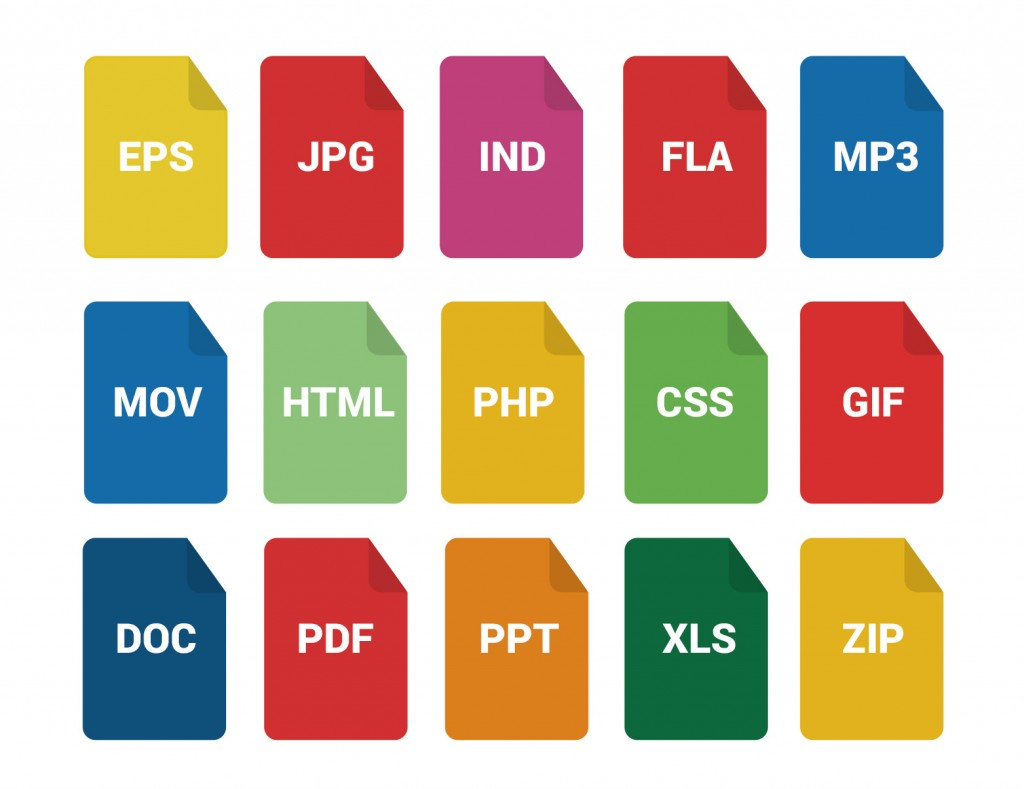
\includegraphics[width=0.4\textwidth]{devcon-files.jpg}
  \transdissolve<3>
 \end{center}
\end{onlyenv}

 \begin{center}
  \begin{tikzpicture}
   \node[chunk,visible on=<3>] at (0,0) (achunk){};
   \node[visible on=<3>] at (-1.8,0) (labeltext){A ``chunk:"};
   \node[chunk,visible on=<3->] at (-4,-3) (a){};
   \node[chunk,visible on=<3->] at (-2,-3) (b){};
   \node[chunk,visible on=<3->] at (0,-3) (c){};
   \node[chunk,visible on=<3->] at (2,-3) (d){};
   \node[chunk,visible on=<3->] at (4,-3) (e){};

   \node at (-4.2,-1.3) (dummy1) {};
   \node at (4.2,-1.7) (dummy2) {};
   \node[chunk,fit=(dummy1)(dummy2),visible on=<5>]{};

   \node[scale=0.8,draw,visible on=<4-5>] at (-4,-1.5) (ha){$h_1$}
     (a.north) edge[-,visible on=<4>] (ha.south);
   \node[scale=0.8,draw,visible on=<4-5>] at (-2,-1.5) (hb){$h_2$}
     (b.north) edge[-,visible on=<4>] (hb.south);
   \node[scale=0.8,draw,visible on=<4-5>] at (0,-1.5) (hc){$h_3$}
     (c.north) edge[-,visible on=<4>] (hc.south);
   \node[scale=0.8,draw,visible on=<4-5>] at (2,-1.5) (hd){$h_4$}
     (d.north) edge[-,visible on=<4>] (hd.south);
   \node[scale=0.8,draw,visible on=<4-5>] at (4,-1.5) (he){$h_5$}
     (e.north) edge[-,visible on=<4>] (he.south);

   \node[chunk,visible on=<6>] at (0,-1.5) {};
     \end{tikzpicture}

 \end{center}
\end{overlayarea}
\end{frame}

\begin{frame}
\begin{overlayarea}{\textwidth}{10cm}

 \begin{columns}[T]
  \begin{column}{0.5\textwidth}
  Chunks are assembled in a \textbf{Merkle Tree}.
  \small
    \begin{itemize}
     \item<1->{Files are retrievable using a single 32byte hash.}
     \item<2->{Built-in integrity protection and random access.}
     \item<3->{Merkle-proofs enable proof-of-custody schemes.}
     \item<4->{Treversible using ASCII charactes due to branching factor of 128.}
    \end{itemize}

  \end{column}
  \begin{column}{0.5\textwidth}
   \only<1-2>{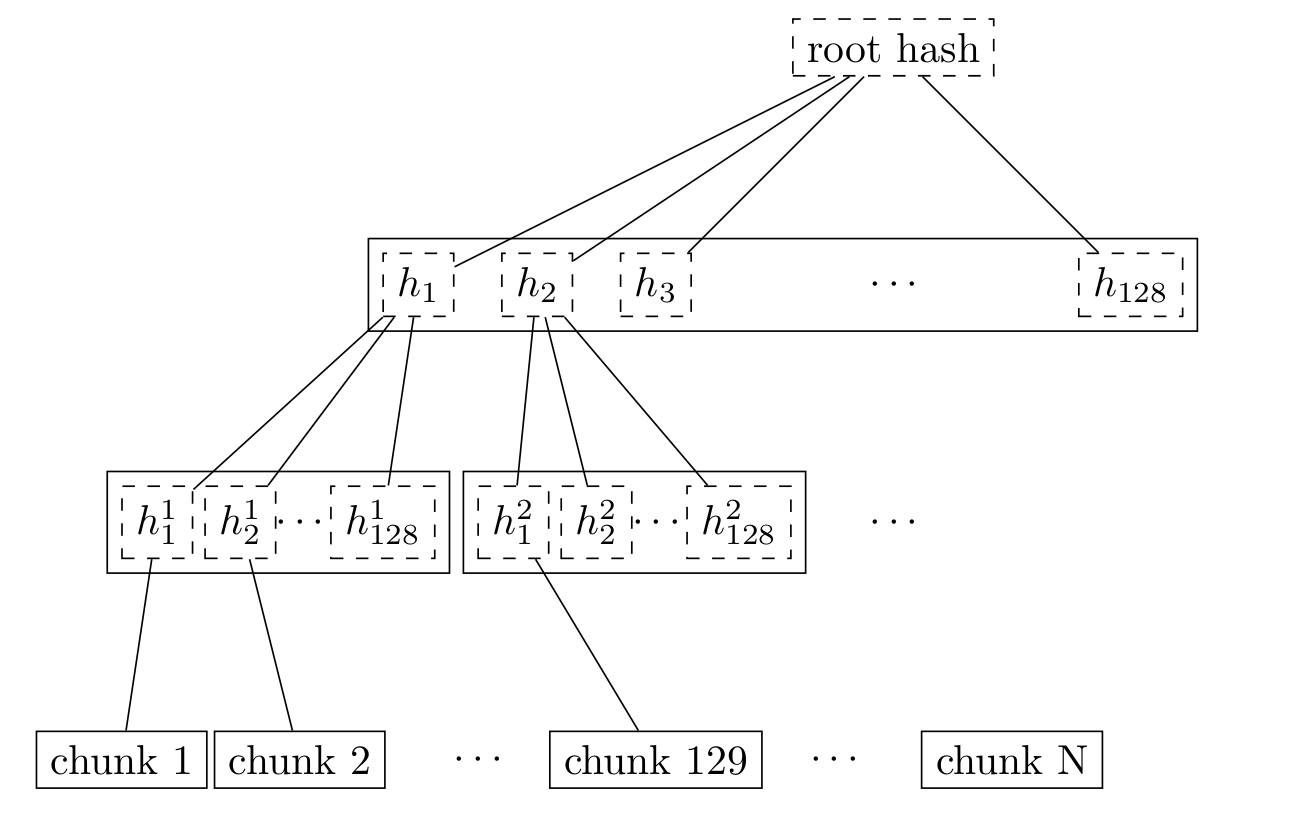
\includegraphics[width=6cm]{devcon-merkle-tree.png}}
   \only<3>{
   \begin{tikzpicture}
    \node[scale=0.4] {
    \documentclass[border=2pt,draw]{standalone}
\usepackage{tikz}
\usetikzlibrary{fit}
\begin{document}

\tikzset{
level/.style={
  sibling distance={(width("$H^126$")+4pt)},
  level distance=15mm,
  line width=.5pt,
},
mtnode/.style={
  minimum width={width("$H^126$")+2pt},
  minimum height={.7cm},
  inner sep=2pt,
  outer sep=2pt,
  rectangle,
  rounded corners=1pt,
  draw,
},
% edge from parent/.style={draw=none},
mtedge/.style={grow=down,draw=none,<-, edge from parent/.style={draw}},
link/.style={draw=none, edge from parent/.style={draw=none}},
mtedgeadj/.style={mtedge, shorten >=10pt  },
mpedge/.style={mtedge, line width=.7pt,densely dashed},
ellip/.style={draw,loosely dotted, shorten >=5mm, thick,<-, edge from parent/.style={draw}},
bubble/.style={minimum height={1cm}, draw=none, align=center},
data/.style={mtnode, fill=gray!50},
mppath/.style={mtnode,dashed,line width=.7pt,fill=gray!30},
mpext/.style={mtnode,line width=.7pt,fill=gray!40},
mpdata/.style={data,line width=.7pt,fill=gray!70},
mpdataext/.style={data,line width=.7pt,fill=gray!80},
}

\begin{tikzpicture}
                  % level 7
\node[mtnode] (root) {$H^7_0$}
                  % level 6
  child[<-,grow=right,level distance=3cm] { node[bubble] (ash) {root-hash}  }
  % child[link,grow=left,level distance=5cm] { node[bubble] (ash) {audit secret}  }
  child { node[mppath] (6-0) {$H^6_0$}   % 0
                  % level 5
    child { node[mppath] (5-0) {$H^5_0$}          % 0
      % child[mpedge]
                  % level 4
                  % mppath goes the other way
      child { node[mpext] (4-0) {$H^4_0$}
        % % child[mtedgeadj]
                  % level 3
        child { node[mtnode] (3-0) {$H^3_0$}
              % level 2
          child { node[mtnode] (2-0) {$H^2_0$}
                % level 1
            child { node[mtnode] (1-0) {$H^1_0$}
                % level 0
              child { node[mtnode] (0-0) {$H^0_0$}
                % data level
                child[mtedge] { node[data] (c-0) {$c_0$} }
              }
              % % child[mtedgeadj]
              child { node[mtnode] (0-1) {$H^0_1$}
                % data level
                child[mtedge] { node[data] (c-1) {$c_1$} }
              }
                % level 0
            }
                % level 1
            % child[mtedgeadj]
            child { node[mtnode] {$H^1_{1}$} child[ellip] }
          }
                % level 2
          % child[mtedgeadj]
          child { node[mtnode] {$H^2_{1}$} child[ellip] }
        }
                % level 3
        % child[mtedgeadj]
        child { node[mtnode] {$H^3_{1}$} child[ellip] }
      }
                % level 4
      child[missing]
      child[missing]
      child { node[mppath] (4-1) {$H^4_1$}                 % 1
                % level 3
        child { node[mpext] (3-4) {$H^3_4$} child[ellip] }
        % child[mpedge]
        child { node[mppath] (3-5) {$H^3_5$}  % 1
                % level 2
          % child[mpedge]
          child { node[mppath] (2-10) {$H^2_{10}$}           % 0
                % level 1
            child { node[mpext] (1-21) {$H^1_{21}$} child[ellip] }
            % child[mpedge]
            child { node[mppath] (1-22) {$H^1_{22}$}         % 1
                % level 0
              child { node[mppath] (0-42) {$H^0_{42}$}       % 0
                % data level
                child[mtedge] { node[mpdata] (c-42) {$c_{42}$} }    % <- pivot
              }
                % level 0
              % child[mpedge]
              child { node[mpext] (0-43) {$H^0_{43}$}
                % data level
                child[mtedge] { node[mpdataext] (c-43) {$c_{43}$} }    % <- neighbo
              }
                % level 0
            }
                % level 1
          }
                % level 2
          % child[mpedge]
          child { node[mpext] (2-11) {$H^2_{11}$} child[ellip] }
        }
                % level 3
        % child[missing]
      }
                % level 4
    }
                % level 5
    child[missing]
    % child[mpedge]
    child[missing]
    child { node[mpext] (5-1) {$H^5_1$} child[ellip] }
  }
                % level 6
  child[missing]
  child[missing]
  % child[mtedgeadj]
  child[missing]
  child  { node[mpext] (6-1) {$H^6_1$}
                % level 5
    child { node[mtnode] (5-2) {$H^5_2$} child[ellip] }
    child[missing]
    % child[mtedgeadj]
    child { node[mtnode] (5-3) {$H^5_3$}
                % level 4
      child { node[mtnode] {$H^4_{6}$} child[ellip] }
      % child[mtedgeadj]
      child { node[mtnode] (4-7) {$H^4_7$}
                % level 3
        child { node[mtnode] {$H^3_{14}$} child[ellip] }
        % child[mtedgeadj]
        child { node[mtnode] (3-15) {$H^3_{15}$}
                % level 2
          child { node[mtnode] {$H^3_{30}$} child[ellip] }
          % child[mtedgeadj]
          child { node[mtnode] (2-31) {$H^2_{31}$}
                % level 1
            child { node[mtnode] {$H^1_{62}$} child[ellip] }
            % child[mtedgeadj] {node {}}
            child { node[mtnode] (1-63) {$H^1_{63}$}
                % level 0
              child { node[mtnode] (0-126) {$H^0_{126}$}
                child[mtedge] { node[data] (c-126) {$c_{126}$} }
              }
              % child[mtedgeadj]
              child { node[mtnode] (0-127) {$H^0_{127}$}
                child[mtedge] { node[data] (c-127) {$c_{127}$} }
              }
                % 0
            }
                % 1
          }
                % 2
        }
                % 3
      }
                % 4
    }
               % 5
  }
               % 6
 ;
\end{tikzpicture}
\end{document}
    };
   \end{tikzpicture}
   }
   \only<4>{
     \begin{tikzpicture}
      \node[scale=0.6] {
         \begin{tikzpicture}
	  \node[draw,dashed] (root) at (5,3) {hash of chunk $h_1$ - $h_{128}$};
	  \node[draw,dashed] (h1) at (1,1) {$h_1$};
	  \node[draw,dashed] (h2) at (2,1) {$h_2$};
	  \node[draw,dashed] (h3) at (3,1) {$h_3$};
	  \node (dots) at (5,1) {$\cdots$};
	  \node[draw,dashed] (h128) at (7,1) {$h_{128}$};
	  % \node[draw,fit=(h1) (h2) (h3) (dots) (h128)]{};
	  \draw (root) -- (h1);
	  \draw (root) -- (h2);
	  \draw (root) -- (h3);
	  \draw (root) -- (h128);
      \end{tikzpicture}
      };
      \end{tikzpicture}
      }
  \end{column}
 \end{columns}

\end{overlayarea}
\end{frame}

\begin{frame}{Manifests}
 We can take this one step further, be tying together various swarm assets under a new root-hash by generating a new tree: A \textbf{Manifest}.\\
 \begin{block}{A Swarm Manifest...}
  ...is a Merkle tree whose leaves are root-hashes of other swarm assets (files, collections, manifests, chunks...)
 \end{block}
 The only difference between this and the chunk-tree of a file, is that it is not balanced and has metadata.
\end{frame}

\begin{frame}
 For example, \uncover<2->{the Swarm landing page
 \begin{center}
  \texttt{swarm-gateways.net/bzz:/swarm/}
 \end{center}
 }
 \end{frame}

\begin{frame}
 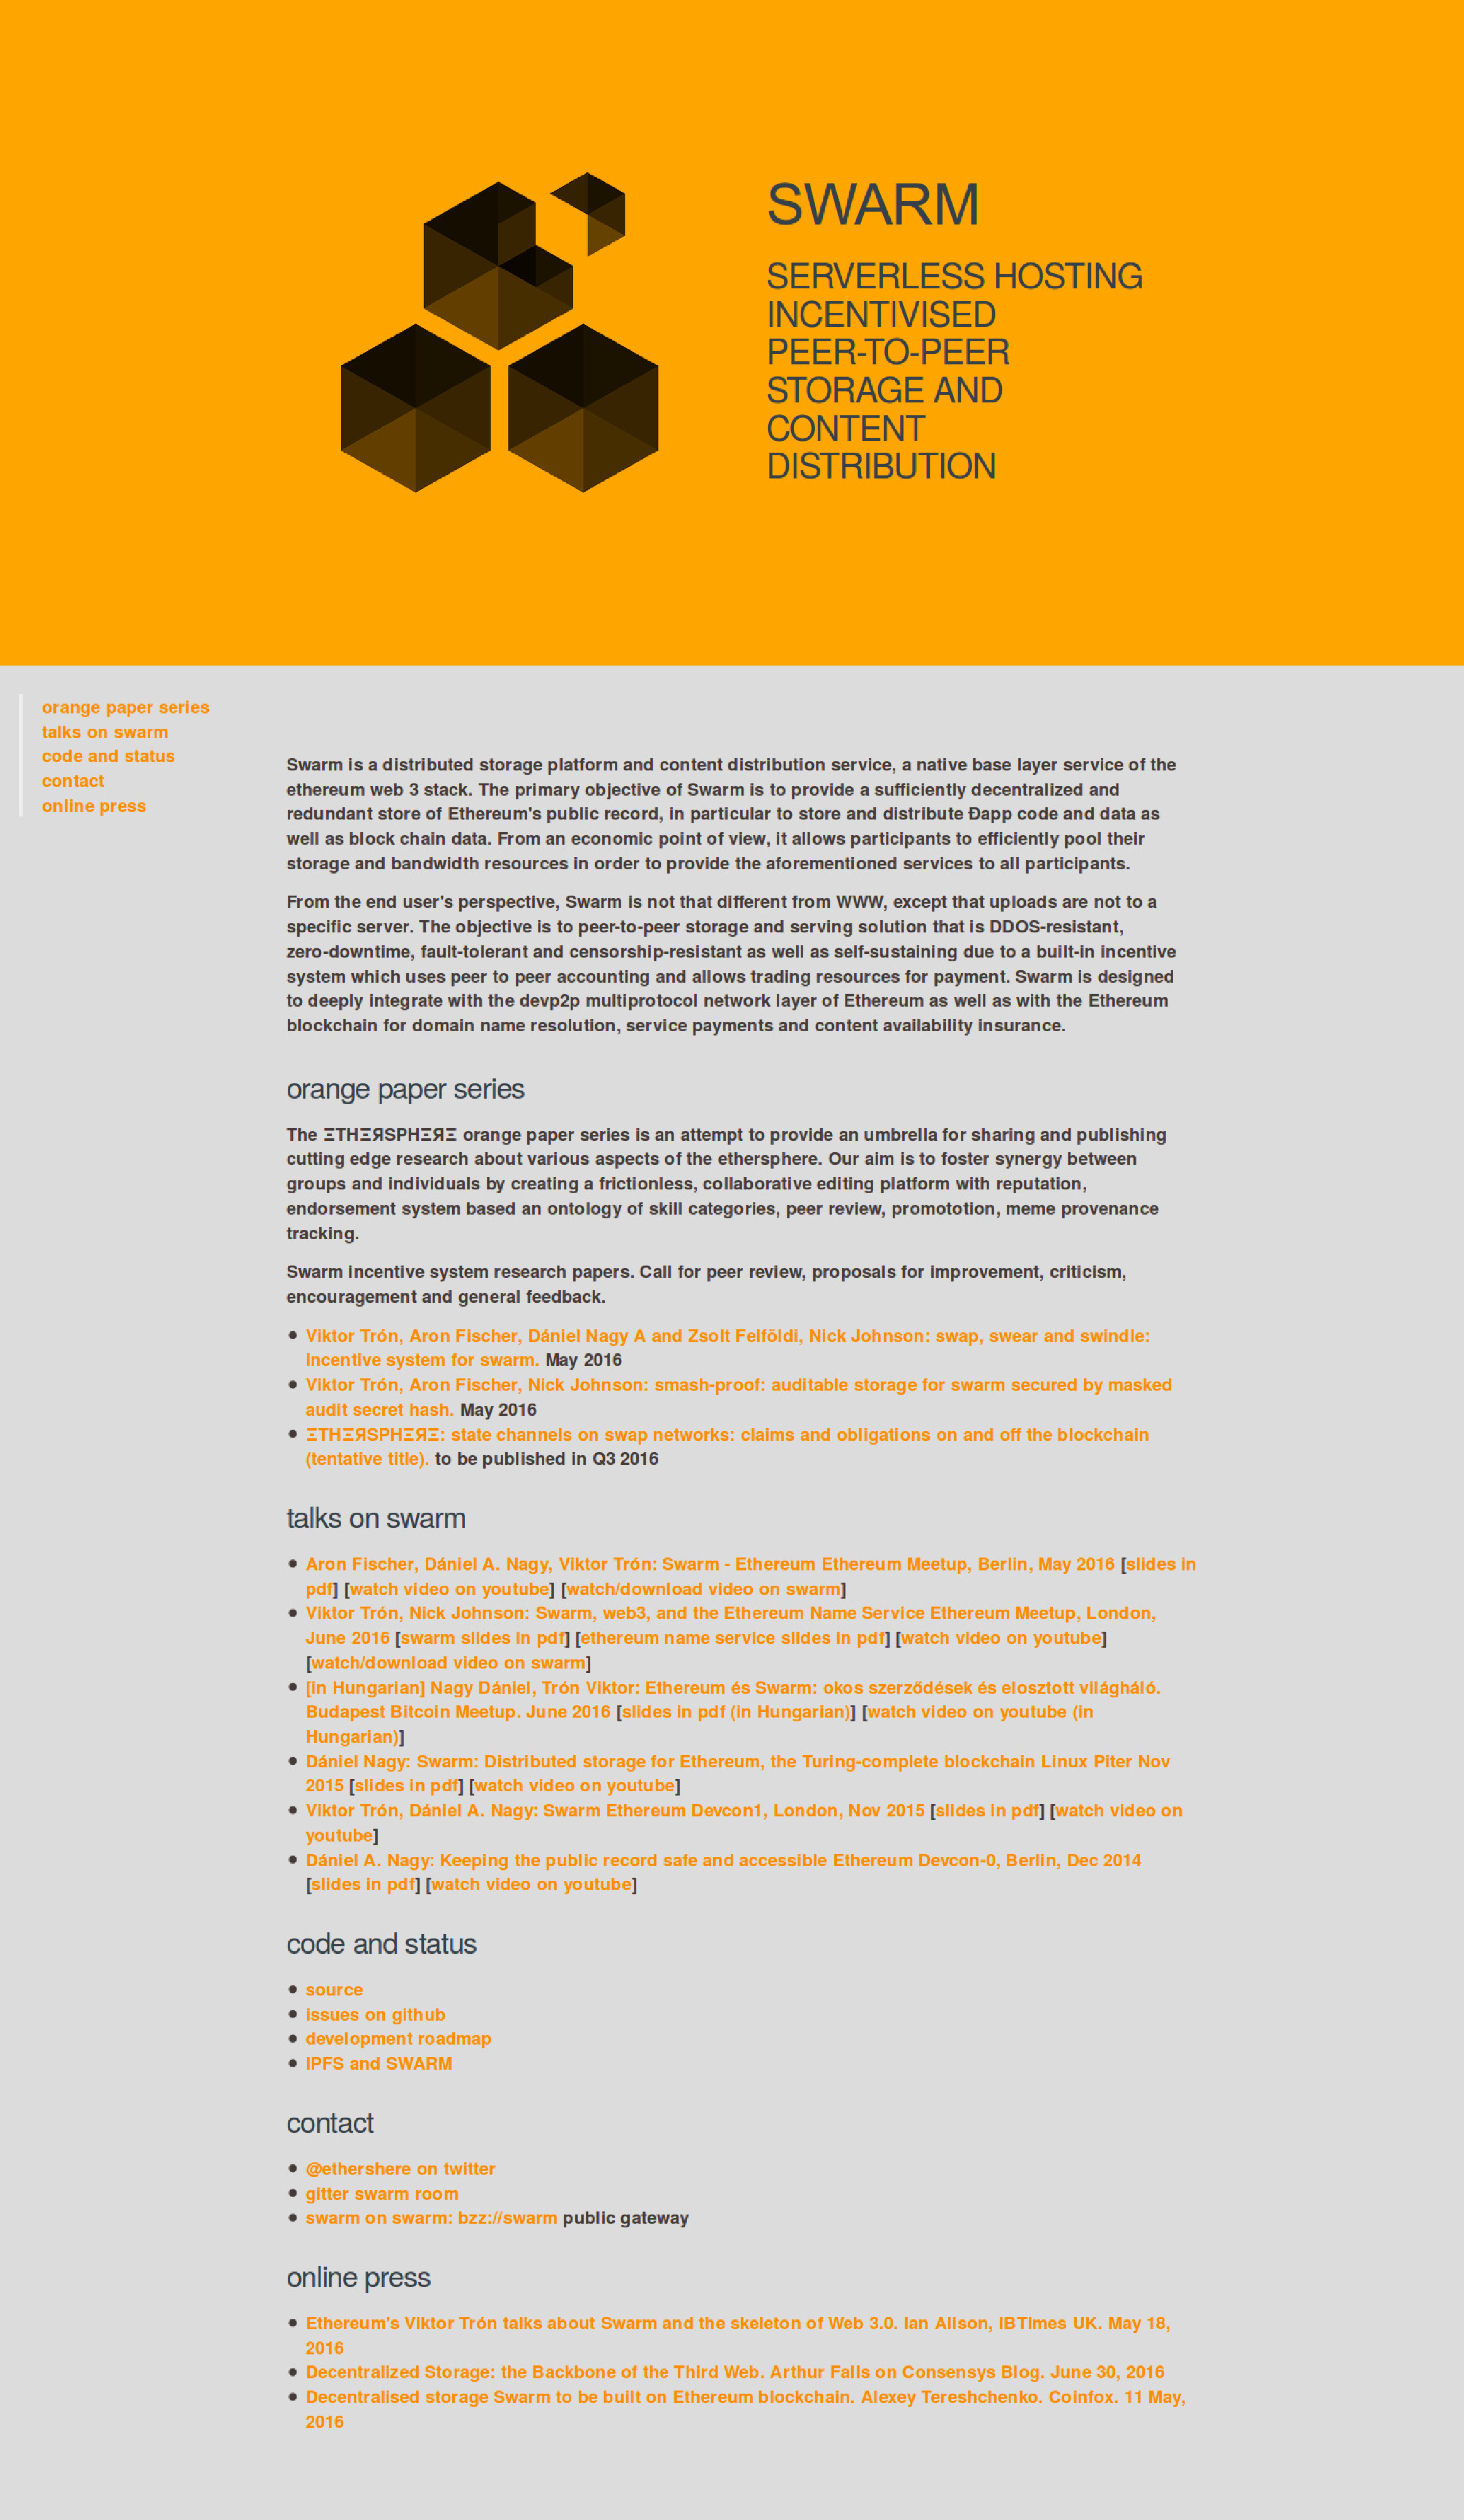
\includegraphics[width=0.8\textwidth]{devcon-swarmsite.pdf}
\end{frame}

\begin{frame}[fragile]
\frametitle{Manifests}
 ...is loaded from this 4-entry manifest:\\
\tiny
\begin{semiverbatim}
\{"entries":[\{
"path":"Swarm_files/",
"hash":"0294e48456a49fe7c02162c83b068075ff9ae6aaafb46439dba32da7de548379",
"contentType":"application/bzz-manifest+json",
"status":0\},
\{"path":"ethersphere/orange-papers/"...
\{"path":"i"...
\{"path":"talks/"...
\{"path":"",
"hash":"6fac0b0c1f118f7f383792c0f01c80d1b2dc94f0e166d62ff4f999a926e9d94a",
"contentType":"text/html;charset=utf-8","status":0\}]\}\end{semiverbatim}
\uncover<2->{\small
 Manifests translate a URL path into swarm hashes (URL defines manifest merkle-tree traversal).\\[2mm]
 When combined with the Ethereum Name Service (ENS) to register a name for the manifest's own root hash, we can \textbf{serve any and all swarm data directly to your browser using human readable names}.
}
\end{frame}

\begin{subsection}{Example: Swarm File Manager}
 \begin{frame}
  With manifests, you can navigate swarm just like you would navigate your own filesystem.\\
  \uncover<2->{Let us open the swarm landing page in the swarm file manager:\\}
  \uncover<3->{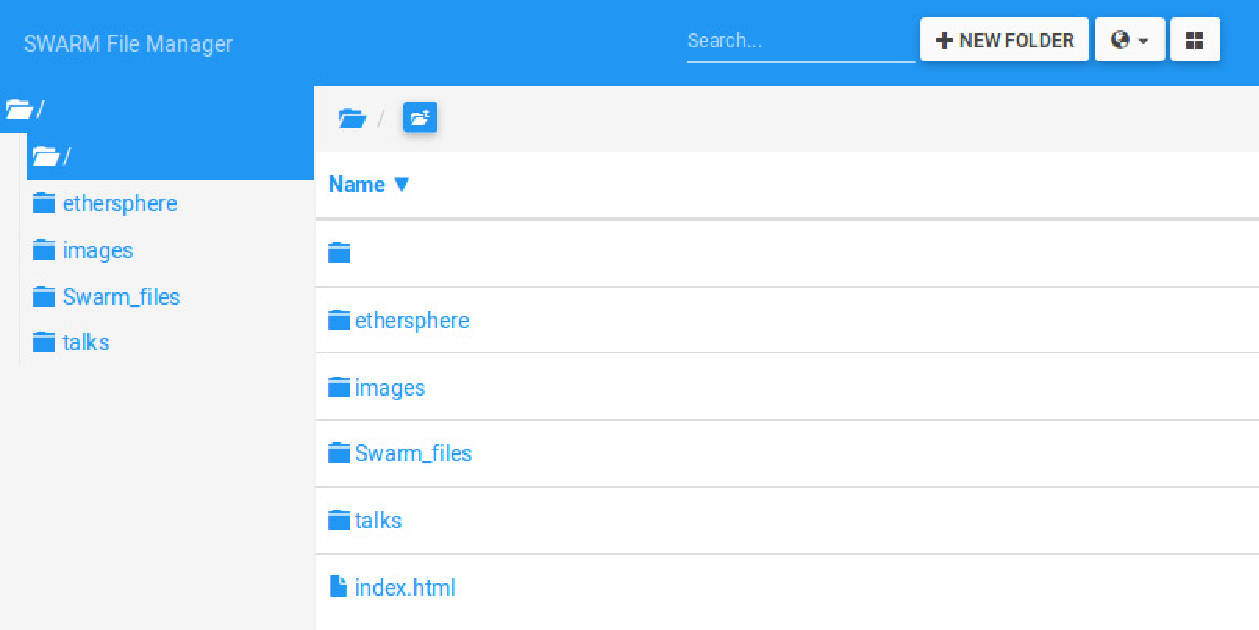
\includegraphics[width=11cm]{devcon-swarmfilemanager.pdf}}
 \end{frame}
\end{subsection}


\begin{subsection}{Manifest Uses}

\begin{frame}

\begin{block}{Using Manifests...}
\begin{itemize}
 \item Two-way translation possible from directories to manifests
  \begin{itemize}
   \item Filesystem API
   \item Dropbox, rsync, ...
   \item Filesystem driver (fuse)
  \end{itemize}
 \item Only root hashes must be registered (ENS) on blockchain. Beyond this the whole site is integrity protected.
 \item Metadata for any manifest entry can include
    \begin{itemize}
      \item copyright information
      \item access control
      \item payment triggers
      \item auto-play continuation
      \item subscription information
      \item database layout info
    \end{itemize}
 \item Version control system (mango = git over swarm)
\end{itemize}
\end{block}

\end{frame}
\end{subsection}



\end{section}

\begin{section}{Dynamic data}
 

\begin{subsection}{Internode communication}

\begin{frame}
 \begin{block}{How does information (dynamic content) move around?}
 Using the same routing and incentive system as storage and retrieval.
 \end{block}
\end{frame}


\begin{frame}{Internode communication}
\begin{block}{What kinds of interactions are we used to?}
 \begin{itemize}
    \item tweets, status updates (public or restricted)
    \item chatroom, discussion forum, stackoverflow
    \item pager \& fax, phonecall, videocall
    \item audio-video broadcast, tv, radio, podcast (live or recorded)
    \item rss, subscription, notifications, newsletters
    \item file transfer, download
 \end{itemize}
\end{block}
\begin{block}<2->{Question:}
 Why are these services provided by private entities and are not part of the basic public infrastructure? After all, everything is just pulling, pushing and storing data.
\end{block}
\end{frame}

\begin{frame}
\setbeamercovered{transparent}% Dim out "inactive" elements
\begin{overlayarea}{\textwidth}{10cm}
To replicate services we are used to, specify storage and delivery criteria.
\begin{block}{}
 \begin{itemize}
  \item<2-> Who is it for?
  \item<3-> How should it be stored and transported?
  \item<4-> Encryption?
  \item<5-> What is the context?
 \end{itemize}
\end{block}
 \only<2->{
\begin{block}<2->{}
\begin{itemize}
  \only<2>{
    \item Is it addressed to specific recipients?
    \item Should it be (re-)delivered to specific recipients?
    }
 \only<3>{
    \item Should it be stored (at content address) or is it ephemeral?
    \item Does it have high priority, is it urgent, is latency a factor?
    \item Should it be archived? is it insured? expiring?
    \item Is data access recorded/receipted?
    }
 \only<4>{
    \item Is it confidential? Private?
    }
 \only<5>{
    \item reaction to previous communication, content, topic? Comments, answers, corrections
    \item Existing asset (reference), streaming data, real time feed?
    \item How should the data be displayed? Timeline or thematic/threaded view
    }
\end{itemize}
\end{block}
}
\end{overlayarea}
\end{frame}


\begin{frame}
 \begin{block}{The Vision}
Use the message routing and content delivery system that swarm uses
 \end{block}
 \begin{block}<2->{Tools at our disposal}
  \begin{itemize}
   \item incentivised message relay (store requests sent towards non-content address must be paid for)
   \item deterministic routing and message delivery (to complement Whisper)
   \item priority queues
   \item insured storage
   \item taking receipts
   \item multicast broadcast
  \end{itemize}
 \end{block}
\end{frame}

\wholeslide{\textbf{PSS}: \textbf{P}ostal \textbf{S}ervices \textbf{S}uite (BZZ-whispered)}

\end{subsection}

\begin{subsection}{Multimedia live broadcast}

\blockslide{}{How can this handle live multimedia sessions?}

\begin{frame}{}
\begin{block}{Multimedia live broadcast: multibitrate low-latency streaming}
 \begin{itemize}
    \item leech - continuous data stream from peers
    \item non-multiplexed multi-bitrate stream offered
    \item RTSP/MPEG-DASH standard - available in most browsers using html5 video tag
    \item webRTC or FFMEG to capture and encode streams
    \item multicast tree - solves scalability of media server solutions
    \item p2p symmetry: the same technique for videoconference or even one-on-one AV session
    \item data goes to viewers via pairwise transmission channels
    \item peers sit on the multicast chain and get  promoted, demoted depending on payment and latency/throughput
    \item the same framework can drive historical syncing
\end{itemize}
\end{block}
\end{frame}

\wholeslide{\textbf{SWATCH}: \textbf{S}treaming \textbf{W}ith \textbf{A}daptive \textbf{T}ransmission \textbf{CH}annels}

\end{subsection}

\begin{subsection}{Database services}


\begin{frame}
\begin{block}{Where is information (dynamic content) pulled from?}
\begin{enumerate}
\item the blockchain, ethereum state \& contract storage. (expensive and slow)
\item local storage private to user, cookies (limited to data only client uses)
\item distributed database on swarm? (cheap and verifiable)
\end{enumerate}
\end{block}
\end{frame}

\begin{frame}
\setbeamercovered{transparent}% Dim out "inactive" elements
\begin{overlayarea}{\textwidth}{10cm}
\begin{block}{How are database services organised?}
\begin{itemize}
\item<1-> Structure
\item<2-> Security
\item<3-> Scalability
\item<4-> Sustainability
\end{itemize}
\end{block}
\begin{block}{How?}
\begin{itemize}
\only<1>{
\item manifests implement key-value store (Patricia Merkle Trie as oppose to traditional DHT)
\item supports various indexes and iteration (range queries)
\item conventions for index entry
\item db table layout manifest
\item linked to ENS
}
\only<2>{
\item  verifiable on the blockchain by challange so it does not have to be on-chain
\item  verifiable authentication, record updates and notifications
}
\only<3>
{
\item sql resolver (reql of rethinkdb) sitting on top
\item parallel processess walk the indexes and merge results
\item index updates, derivative data (full text search indexes, aggregate statistics) supplied by a computational market
\item query caching and accelerated retrieval for real-time low latency experience supplied by specialised nodes
}
\only<4>
{q
\item due to verifiable computations (truebit, ewasm), \textit{swap, swear and swindle} is applicable
\end{itemize}
\end{block}
\begin{block}{Examples}
\begin{itemize}
\item example: decentralised markets
\item example: storing the blockchain and state on swarm
}
\end{itemize}
\end{block}
\end{overlayarea}
\end{frame}

\wholeslide{\textbf{SWORD}: \textbf{S}tate \textbf{W}ith \textbf{O}n-demand \textbf{R}etrieval of \textbf{D}ata}


\begin{frame}
\begin{block}{Can we put the ethereum blockchain and state on swarm}
\begin{itemize}
 \item light client, LES protocol abstraction - flexible transition from remote, light, full and archival nodes
 \item solves the scalability problem of too big state data, receipts, contract storage, fast syncing
 \item decentralised blockchain explorer
\end{itemize}
\end{block}
\end{frame}

\end{subsection}



\begin{subsection}{Current Status}
\begin{frame}[plain]
 \begin{tikzpicture}
  \node[scale=1]{
  \begin{tikzpicture}
  \node[anchor=center] at (current page.center) (thepic){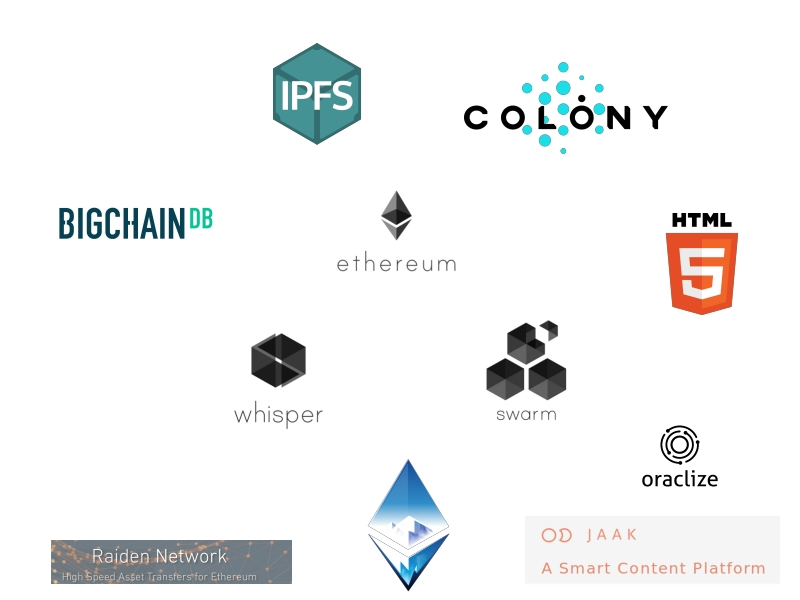
\includegraphics[width=0.9\textwidth]{ecosystem1.jpg}};
  \node[below=1cm of thepic.130] {\textbf{PSS}};
  \node[below=5cm of thepic.135] {\textbf{ENS}};
  \node[below=2.7cm of thepic.65] {\textbf{SWATCH}};
  \end{tikzpicture}
 };
 \end{tikzpicture}

\end{frame}


\begin{frame}{Ethereum: status and roadmap}
 \begin{block}{Current Status}
 `Homestead' up and running. Multiple client implementations.
 \end{block}
 \begin{block}{Roadmap}
  `Metropolis' release milestone\\
  `Mist browser' - Dapp browser with swarm support.
 \end{block}

\end{frame}


\begin{frame}{Swarm: status and usage}
\begin{block}<1->{What is the developlent status of swarm?}
\begin{enumerate}
\item golang implementation: proof-of-concept iteration 2 release 4, code has been merged to go-ethereum develop branch
\item Microsoft Azure hosting a testnet of 100+ nodes
\item expanding team, come join or contribute
\end{enumerate}
\end{block}

\begin{block}<2->{How can swarm be used?}
\begin{itemize}
\item bzzd - swarm daemon, communicates with ethereum via IPC, so any ethereum client works
\item APIs: JSON RPC (via websockets, http, or ipc), http proxy, cli, fuse driver (planned)
\item API bindings: web3.js and CLI
\end{itemize}
\end{block}

\end{frame}

\begin{frame}
\begin{overlayarea}{\textwidth}{10cm}
\begin{tikzpicture}
\node[scale=0.8] at (current page.center) {
\begin{tikzpicture}

 \node[draw,rounded corners] at (4,4) (goapi) {
\includegraphics[width=2cm]{golang.png} API};

 \node[draw,rounded corners] at (0,0) (ipc) {JSON IPC};
 \node[draw,rounded corners] at (4,0) (proxy) {http-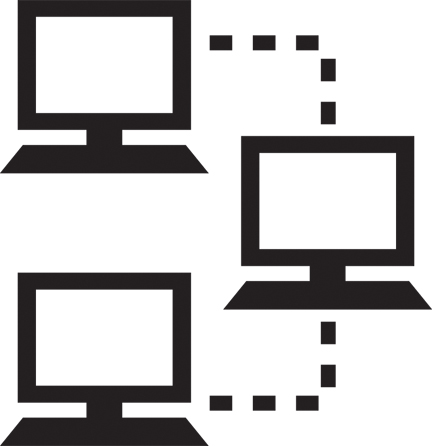
\includegraphics[width=1cm]{proxy.jpg}-proxy};
 \node[draw,rounded corners] at (8,0) (fuse) {fuse 
\includegraphics[width=1cm]{fuse.jpg}};

 \node[draw,rounded corners] at (2,-4) (cli) {CLI 
\includegraphics[width=1cm]{cli.png}};
 \node[draw,rounded corners] at (6,-4) (web3js) {web3.js};

 \node {}
 (cli) edge[point,->] (ipc)
 (web3js) edge[point,->] (ipc)
 (cli) edge[point,->] (proxy)
 (web3js) edge[point,->] (proxy)
 (cli) edge[point,->] (fuse)
 (web3js) edge[point,->] (fuse)
 (ipc) edge[point,->] (goapi)
 (proxy) edge[point,->] (goapi)
 (fuse) edge[point,->] (goapi)
 ;
\end{tikzpicture}
};
\end{tikzpicture}
\end{overlayarea}
\end{frame}

\end{subsection}



\end{section}

\begin{frame}[plain]{Join us}

\begin{block}<1->{Contact and contribute}
\begin{itemize}
\item swarm channel: \texttt{https://gitter.im/ethereum/swarm}
\item orange papers \texttt{http://web3.download/bzz:/swarm/}
\item join our research channel, reading group and write the orange papers \texttt{https://gitter.im/ethersphere/orange-lounge}
\end{itemize}
\end{block}
\begin{block}{The Team}
\begin{itemize}
\footnotesize
\item Daniel A. Nagy, Nick Johnson, Viktor Trón (Zsolt Felföldi) (core team)
\item Ram Devish, Bas van Kervel, Alex van der Sande (Mist integration)
\item Felix Lange (integration, devp2p)
\item Igor Shadurin (file manager dapp)
\item Aron Fischer \& Ethersphere orange lounge group
\item Nick Johnson, Alex van der Sande (Ethereum Name Service)
\item Gavin Wood, Vitalik Buterin, Jeffrey Wilcke (visionaries)
\end{itemize}
\end{block}

\end{frame}



\end{document}
